\chapter{Numerical Sequences \& Convergence}
\label{chap:sequences}

\section{The Limit Concept and the $\varepsilon$-$N$ Definition}

A \textbf{numerical sequence} of real numbers is a mapping from the natural numbers into the reals:
\[
u: \mathbb{N} \longrightarrow \mathbb{R}, \qquad n \longmapsto u(n) \equiv u_n.
\]
We denote the entire sequence by $(u_n)_{n \in \mathbb{N}}$ or simply $(u_n)$.

\begin{figure}[htbp]
  \centering
  \begin{minipage}{0.35\textwidth}
    \centering
    
\includegraphics[width=0.82\textwidth]{cauchy.jpg}
    \caption*{(a) \textbf{Augustin-Louis Cauchy (1789--1857)}}
  \end{minipage}
  \hspace{0.08\textwidth}
  \begin{minipage}{0.35\textwidth}
    \centering
    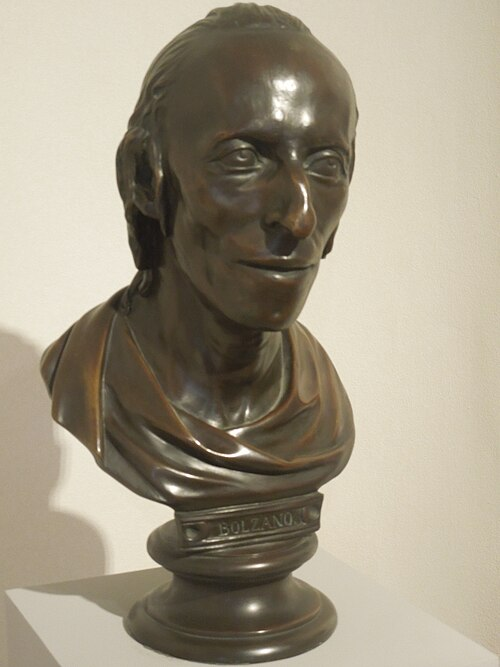
\includegraphics[width=0.82\textwidth]{bolzano.jpg}
    \caption*{(b) \textbf{Bernard Bolzano (1781--1848)}}
  \end{minipage}
  \caption{\textbf{Architects of Modern Rigorous Analysis:} Augustin-Louis Cauchy (who formalized $\varepsilon$-$\delta$ limits, continuity, and Cauchy sequences) and Bernard Bolzano (pioneer of the Bolzano-Weierstrass theorem and intermediate value theorem).}
  \label{fig:cauchy_bolzano}
\end{figure}

\begin{definitionbox}{Convergence of a Sequence ($\varepsilon$-$N$ Formulation)}
A sequence $(u_n)$ is said to \textbf{converge} to a finite real limit $l \in \mathbb{R}$, denoted $\lim_{n \to \infty} u_n = l$ or $u_n \xrightarrow[n \to \infty]{} l$, if:
\begin{equation}
\forall \varepsilon > 0, \quad \exists N_\varepsilon \in \mathbb{N} \quad \text{such that} \quad \forall n \in \mathbb{N}, \quad \left( n > N_\varepsilon \implies |u_n - l| < \varepsilon \right).
\end{equation}
Equivalently: for every interval $(l - \varepsilon, l + \varepsilon)$ centered on $l$, all terms of the sequence from index $N_\varepsilon + 1$ onward lie strictly inside the interval. A sequence that does not converge is called \textbf{divergent}.
\end{definitionbox}

\begin{figure}[htbp]
  \centering
  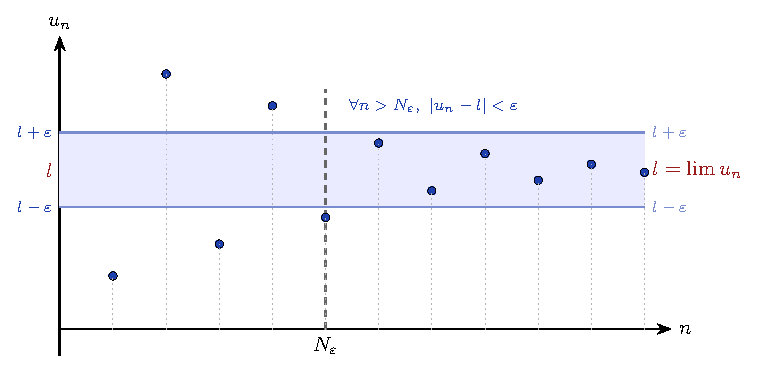
\includegraphics[width=0.90\textwidth]{04_sequence_convergence.pdf}
  \caption{\textbf{Geometric Interpretation of Sequence Convergence:} Given an arbitrary tolerance $\varepsilon > 0$, an index $N_\varepsilon$ exists such that for all indices $n > N_\varepsilon$, all sequence points $u_n$ are permanently trapped within the horizontal $\varepsilon$-tube $(l - \varepsilon, l + \varepsilon)$.}
  \label{fig:seq_convergence}
\end{figure}

\begin{theorembox}{Uniqueness of the Limit and Boundedness}
\begin{enumerate}[leftmargin=1.4em,itemsep=3pt]
  \item \textbf{Uniqueness:} If a sequence $(u_n)$ converges, its limit $l$ is \textbf{unique}:
  \[
  (u_n \to l_1 \quad \text{and} \quad u_n \to l_2) \implies l_1 = l_2.
  \]
  \item \textbf{Boundedness:} Every convergent sequence is \textbf{bounded}:
  \[
  (u_n \to l) \implies \exists M > 0, \quad \forall n \in \mathbb{N}, \quad |u_n| \le M.
  \]
  (\textit{Note:} The converse is false; e.g. $u_n = (-1)^n$ is bounded but divergent).
\end{enumerate}
\end{theorembox}

\begin{definitionbox}{Infinite Limits and Divergence to Infinity}
\begin{enumerate}[leftmargin=1.4em,itemsep=2pt]
  \item $\lim_{n \to \infty} u_n = +\infty \iff \forall A > 0, \ \exists N_A \in \mathbb{N}, \ \forall n > N_A, \ u_n > A$.
  \item $\lim_{n \to \infty} u_n = -\infty \iff \forall B > 0, \ \exists N_B \in \mathbb{N}, \ \forall n > N_B, \ u_n < -B$.
\end{enumerate}
\end{definitionbox}

\section{Fundamental Convergence Criteria}

\begin{theorembox}{The Squeeze (Sandwich / Gendarmes) Theorem}
Let $(u_n), (v_n), (w_n)$ be three real sequences such that:
\begin{enumerate}[leftmargin=1.4em,itemsep=2pt]
  \item There exists an integer $n_0 \in \mathbb{N}$ such that $\forall n \ge n_0, \ v_n \le u_n \le w_n$;
  \item $\lim_{n \to \infty} v_n = \lim_{n \to \infty} w_n = l$.
\end{enumerate}
Then the sequence $(u_n)$ converges and its limit is:
\begin{equation}
\lim_{n \to \infty} u_n = l.
\end{equation}
\end{theorembox}

\begin{theorembox}{The Monotone Convergence Theorem}
\begin{enumerate}[leftmargin=1.4em,itemsep=3pt]
  \item If $(u_n)$ is **monotonically increasing** ($u_{n+1} \ge u_n$) and **bounded above**, then $(u_n)$ converges, and its limit is the supremum of its range:
  \[
  \lim_{n \to \infty} u_n = \sup \{ u_n \mid n \in \mathbb{N} \}.
  \]
  If it is increasing and not bounded above, then $\lim_{n \to \infty} u_n = +\infty$.
  \item If $(u_n)$ is **monotonically decreasing** ($u_{n+1} \le u_n$) and **bounded below**, then $(u_n)$ converges, and its limit is the infimum of its range:
  \[
  \lim_{n \to \infty} u_n = \inf \{ u_n \mid n \in \mathbb{N} \}.
  \]
  If it is decreasing and not bounded below, then $\lim_{n \to \infty} u_n = -\infty$.
\end{enumerate}
\end{theorembox}

\section{Subsequences, Cauchy Sequences, and Adjacent Sequences}

\begin{definitionbox}{Subsequences (Suites Extraites)}
Let $(u_n)_{n \in \mathbb{N}}$ be a sequence. A **subsequence** is a sequence of the form $(u_{\phi(k)})_{k \in \mathbb{N}}$, where:
\[
\phi: \mathbb{N} \longrightarrow \mathbb{N} \quad \text{is a strictly increasing function} \quad (\phi(0) < \phi(1) < \phi(2) < \dots).
\]
Note that for every $k \in \mathbb{N}$, $\phi(k) \ge k$.
If $u_n \to l$, then every subsequence converges to the exact same limit: $u_{\phi(k)} \xrightarrow[k \to \infty]{} l$.
\end{definitionbox}

\begin{theorembox}{The Bolzano-Weierstrass Theorem for Sequences}
Every \textbf{bounded sequence} of real numbers possesses at least one \textbf{convergent subsequence}.
\end{theorembox}

\begin{definitionbox}{Cauchy Sequences and Completeness}
A sequence $(u_n)$ is a \textbf{Cauchy sequence} if its terms become arbitrarily close to each other as their indices grow:
\begin{equation}
\forall \varepsilon > 0, \quad \exists N \in \mathbb{N} \quad \text{such that} \quad \forall p, q \in \mathbb{N}, \quad \left( (p > N \ \land \ q > N) \implies |u_p - u_q| < \varepsilon \right).
\end{equation}
\textbf{The Cauchy Criterion (Completeness of $\mathbb{R}$):}
In the real number field $\mathbb{R}$, a sequence converges to a finite limit if and only if it is a Cauchy sequence:
\[
(u_n) \text{ converges in } \mathbb{R} \iff (u_n) \text{ is a Cauchy sequence}.
\]
\end{definitionbox}

\begin{definitionbox}{Adjacent Sequences (Suites Adjacentes)}
Two sequences $(u_n)$ and $(v_n)$ are said to be \textbf{adjacent} if:
\begin{enumerate}[leftmargin=1.4em,itemsep=2pt]
  \item $(u_n)$ is monotonically increasing;
  \item $(v_n)$ is monotonically decreasing;
  \item $\lim_{n \to \infty} (v_n - u_n) = 0$.
\end{enumerate}
\textbf{Theorem on Adjacent Sequences:}
If $(u_n)$ and $(v_n)$ are adjacent, then:
\begin{itemize}[leftmargin=1.4em,itemsep=1pt]
  \item For all $n \in \mathbb{N}$, $u_n \le v_n$;
  \item Both sequences converge to the **exact same common limit** $l \in \mathbb{R}$:
  \[
  \lim_{n \to \infty} u_n = \lim_{n \to \infty} v_n = l, \qquad \text{and} \quad \forall n \in \mathbb{N}, \quad u_n \le l \le v_n.
  \]
\end{itemize}
\end{definitionbox}

\section{Worked Examples with Step-by-Step Proofs}

\begin{workedexample}{Rigorous Proof of Limit Uniqueness by Contradiction}
Prove from the formal $\varepsilon$-$N$ definition that the limit of a convergent sequence is unique.

\paragraph{Solution and Proof.}
Let $(u_n)$ be a sequence. Assume to the contrary that $(u_n)$ converges to two distinct limits $l_1 \neq l_2$.
Then the distance between them is strictly positive:
\[
|l_1 - l_2| > 0.
\]
Choose $\varepsilon = \frac{|l_1 - l_2|}{2} > 0$.
\begin{enumerate}[leftmargin=1.4em,itemsep=3pt]
  \item Since $u_n \to l_1$, by the definition of limit for this $\varepsilon$, there exists an integer $N_1 \in \mathbb{N}$ such that:
  \[
  \forall n > N_1, \quad |u_n - l_1| < \varepsilon = \frac{|l_1 - l_2|}{2}.
  \]
  \item Since $u_n \to l_2$, there exists an integer $N_2 \in \mathbb{N}$ such that:
  \[
  \forall n > N_2, \quad |u_n - l_2| < \varepsilon = \frac{|l_1 - l_2|}{2}.
  \]
\end{enumerate}
Now choose any index $n_0 > \max(N_1, N_2)$.
For this $n_0$, both inequalities hold simultaneously.
Using the triangle inequality:
\begin{align*}
|l_1 - l_2| &= |(l_1 - u_{n_0}) + (u_{n_0} - l_2)| \\
            &\le |l_1 - u_{n_0}| + |u_{n_0} - l_2| = |u_{n_0} - l_1| + |u_{n_0} - l_2| \\
            &< \frac{|l_1 - l_2|}{2} + \frac{|l_1 - l_2|}{2} = |l_1 - l_2|.
\end{align*}
This yields the strict inequality:
\[
|l_1 - l_2| < |l_1 - l_2|,
\]
which is an undeniable logical contradiction ($x < x$).
Therefore, the assumption that $l_1 \neq l_2$ is false, establishing that:
\[
\mathbf{l_1 = l_2}. \quad \blacksquare
\]
\end{workedexample}

\begin{workedexample}{Verification of Limit via Formal $\varepsilon$-$N$ Argument}
Using the formal $\varepsilon$-$N$ definition of limit, prove that:
\[
\lim_{n \to \infty} \frac{3n + 5}{2n - 1} = \frac{3}{2}.
\]

\paragraph{Solution and Proof.}
Let $\varepsilon > 0$ be given. We must find an integer $N_\varepsilon \in \mathbb{N}$ such that for all $n > N_\varepsilon$:
\[
\left| \frac{3n + 5}{2n - 1} - \frac{3}{2} \right| < \varepsilon.
\]
Compute the algebraic difference over a common denominator:
\[
\frac{3n + 5}{2n - 1} - \frac{3}{2} = \frac{2(3n + 5) - 3(2n - 1)}{2(2n - 1)} = \frac{(6n + 10) - (6n - 3)}{2(2n - 1)} = \frac{13}{2(2n - 1)}.
\]
For $n \ge 1$, $2n - 1 > 0$, so the absolute value can be removed:
\[
\left| \frac{3n + 5}{2n - 1} - \frac{3}{2} \right| = \frac{13}{4n - 2}.
\]
We require:
\[
\frac{13}{4n - 2} < \varepsilon \iff 4n - 2 > \frac{13}{\varepsilon} \iff 4n > \frac{13}{\varepsilon} + 2 \iff n > \frac{13}{4\varepsilon} + \frac{1}{2}.
\]
By the Archimedean property of $\mathbb{R}$, we can choose:
\[
N_\varepsilon = \left\lfloor \frac{13}{4\varepsilon} + \frac{1}{2} \right\rfloor + 1 \in \mathbb{N}.
\]
Then for any $n > N_\varepsilon$:
\[
n > \frac{13}{4\varepsilon} + \frac{1}{2} \implies 4n - 2 > \frac{13}{\varepsilon} \implies \left| \frac{3n + 5}{2n - 1} - \frac{3}{2} \right| = \frac{13}{4n - 2} < \varepsilon.
\]
This completes the formal proof that $\mathbf{\lim_{n \to \infty} \frac{3n + 5}{2n - 1} = \frac{3}{2}}$. $\blacksquare$
\end{workedexample}

\begin{workedexample}{Convergence of a Recurring Sequence via Monotone Convergence}
Consider the sequence $(u_n)_{n \in \mathbb{N}}$ defined by recurrence:
\[
u_0 = 1, \qquad u_{n+1} = \sqrt{2 + u_n} \quad \text{for all } n \ge 0.
\]
\begin{enumerate}[leftmargin=1.4em,itemsep=2pt]
  \item Prove by mathematical induction that for all $n \in \mathbb{N}$, $1 \le u_n < 2$.
  \item Prove by mathematical induction that $(u_n)$ is strictly increasing.
  \item Deduce that $(u_n)$ converges and calculate its limit $l$.
\end{enumerate}

\paragraph{Solution and Proof.}
\textbf{1. Boundedness by Induction ($1 \le u_n < 2$):}
\begin{itemize}[leftmargin=1.4em,itemsep=2pt]
  \item \textbf{Base step ($n = 0$):} $u_0 = 1$, which satisfies $1 \le 1 < 2$. True.
  \item \textbf{Inductive step:} Assume $1 \le u_k < 2$ for some $k \ge 0$.
  Adding $2$: $3 \le 2 + u_k < 4$.
  Since the square root function is strictly increasing on $\mathbb{R}^+$:
  \[
  \sqrt{3} \le \sqrt{2 + u_k} < \sqrt{4} = 2.
  \]
  Since $1 < \sqrt{3} \approx 1.732$, we have $1 \le u_{k+1} < 2$.
\end{itemize}
Thus, by induction, $1 \le u_n < 2$ for all $n \in \mathbb{N}$.

\textbf{2. Monotonicity by Induction ($u_{n+1} > u_n$):}
\begin{itemize}[leftmargin=1.4em,itemsep=2pt]
  \item \textbf{Base step ($n = 0$):} $u_0 = 1$ and $u_1 = \sqrt{2 + 1} = \sqrt{3} \approx 1.732 > 1 = u_0$. True.
  \item \textbf{Inductive step:} Assume $u_{k+1} > u_k$ for some $k \ge 0$.
  Adding $2$: $2 + u_{k+1} > 2 + u_k$.
  Taking square roots:
  \[
  \sqrt{2 + u_{k+1}} > \sqrt{2 + u_k} \implies u_{k+2} > u_{k+1}.
  \]
\end{itemize}
Thus, $(u_n)$ is strictly increasing.

\textbf{3. Convergence and Limit Calculation:}
Because $(u_n)$ is strictly increasing and bounded above by $2$, the **Monotone Convergence Theorem** guarantees that $(u_n)$ converges to a finite limit $l \in [1, 2]$:
\[
\lim_{n \to \infty} u_n = l.
\]
Since the function $f(x) = \sqrt{2 + x}$ is continuous on $[1, 2]$:
\[
\lim_{n \to \infty} u_{n+1} = f\left( \lim_{n \to \infty} u_n \right) \implies l = \sqrt{2 + l}.
\]
Squaring both sides ($l \ge 1 > 0$):
\[
l^2 = 2 + l \implies l^2 - l - 2 = 0 \implies (l - 2)(l + 1) = 0.
\]
The roots are $l = 2$ and $l = -1$.
Since $u_n \ge 1$ for all $n$, the limit must be positive ($l \ge 1$), which rejects $l = -1$.
Therefore:
\[
\mathbf{\lim_{n \to \infty} u_n = 2}. \quad \blacksquare
\]
\end{workedexample}

\begin{workedexample}{Euler's Constant $e$ via Adjacent Sequences}
Define the two sequences for $n \ge 1$:
\[
u_n = \left( 1 + \frac{1}{n} \right)^n, \qquad v_n = \left( 1 + \frac{1}{n} \right)^{n+1}.
\]
\begin{enumerate}[leftmargin=1.4em,itemsep=2pt]
  \item Show that $v_n = u_n \left( 1 + \frac{1}{n} \right)$ and that $\lim_{n \to \infty} (v_n - u_n) = 0$.
  \item Given that $(u_n)$ is strictly increasing and $(v_n)$ is strictly decreasing, prove that $(u_n)$ and $(v_n)$ are adjacent.
  \item Conclude on the existence of Euler's number $e = \lim_{n \to \infty} \left( 1 + \frac{1}{n} \right)^n$ and establish the framing $u_n < e < v_n$.
\end{enumerate}

\paragraph{Solution and Proof.}
\textbf{1. Ratio and Difference:}
\[
v_n = \left( 1 + \frac{1}{n} \right)^{n+1} = \left( 1 + \frac{1}{n} \right)^n \cdot \left( 1 + \frac{1}{n} \right) = u_n \left( 1 + \frac{1}{n} \right).
\]
The difference is:
\[
v_n - u_n = u_n \left( 1 + \frac{1}{n} \right) - u_n = \frac{u_n}{n}.
\]
By the binomial theorem, $u_n = \sum_{k=0}^n \binom{n}{k} \frac{1}{n^k} = 1 + 1 + \frac{1}{2!} \left(1 - \frac{1}{n}\right) + \dots < \sum_{k=0}^\infty \frac{1}{k!} = 3$.
Since $0 < u_n < 3$:
\[
0 < v_n - u_n = \frac{u_n}{n} < \frac{3}{n}.
\]
Taking limits as $n \to \infty$, since $\lim \frac{3}{n} = 0$, by the squeeze theorem:
\[
\lim_{n \to \infty} (v_n - u_n) = 0.
\]

\textbf{2. Adjacency of the Sequences:}
\begin{itemize}[leftmargin=1.4em,itemsep=1pt]
  \item $(u_n)$ is strictly increasing;
  \item $(v_n)$ is strictly decreasing;
  \item $\lim_{n \to \infty} (v_n - u_n) = 0$.
\end{itemize}
All three conditions of the **Adjacent Sequences Theorem** are satisfied.

\textbf{3. Existence and Definition of $e$:}
By the theorem on adjacent sequences, $(u_n)$ and $(v_n)$ converge to a unique common limit, which defines **Euler's number** $e$:
\[
\mathbf{\lim_{n \to \infty} \left( 1 + \frac{1}{n} \right)^n = \lim_{n \to \infty} \left( 1 + \frac{1}{n} \right)^{n+1} = e \approx 2.718\,281\,828\dots}
\]
Furthermore, for every positive integer $n \ge 1$:
\[
\mathbf{\left( 1 + \frac{1}{n} \right)^n < e < \left( 1 + \frac{1}{n} \right)^{n+1}}. \quad \blacksquare
\]
\end{workedexample}
